% !TeX root = ../main.tex

\appendix{A}{附錄名稱}

% appendix body

\begin{figure}[h]
  \centerline{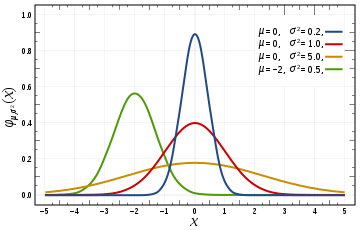
\includegraphics[width=0.5\columnwidth]{gambar}}
  \caption*{附錄圖片}
  \label{figure:apxfig1}
\end{figure}

\begin{table}[h]
    \centering
    \caption*{附錄表格}
    \label{table:apxtab1}
    \begin{tabular}{p{\textwidth/2}p{\textwidth/2}}
        \hline
        \multicolumn{1}{c}{\textbf{硬體}} & \multicolumn{1}{c}{\textbf{軟體}} \\ \hline
        Intel(R) Core(TM) i7-8700 CPU      & Ubuntu 18.04.3 LTS               \\
        NVIDIA GeForce GTX 1080 Ti         & CUDA 10.1                        \\
        DDR4 32GB                          & PyTorch 1.3.1                    \\
        SSD 1TB                            &                                  \\ \hline
    \end{tabular}
\end{table}